\documentclass[12pt]{article}

\usepackage[table]{xcolor}
\usepackage{ccicons}

% Colors
% Page number, etc
\definecolor{meta}{rgb}{0.4,0.4,0.4}

% Palette
\definecolor{s1}{RGB}{130,64,113}
\definecolor{s2}{RGB}{44,109,156}
\definecolor{s3}{RGB}{84,130,43}
\definecolor{s4}{RGB}{231,117,46}
\definecolor{s5}{RGB}{180,66,68}

% Critic
\colorlet{del}{s5}
\colorlet{add}{s3}
\colorlet{hlh}{s4}
\colorlet{not}{s1}

% Accent color
\colorlet{accent}{s2}

% Title background
\definecolor{bg}{RGB}{218, 228, 236}


% pgf
\usepackage{tikz}
\tikzstyle{node}=[draw, circle, minimum size=0.8cm, thick]
\tikzstyle{edge}=[draw, thick]
\usetikzlibrary{arrows}

\usepackage{pgfplots}
\pgfkeys{/pgf/number format/.cd,1000 sep={\,}}
\usepgfplotslibrary{groupplots}

\pgfplotscreateplotcyclelist{scatter cycle}{
    {draw=accent, thin, only marks, mark size = 2.2pt, mark=*, fill=bg},
    {draw=accent, thin, only marks, mark size = 2.2pt, mark=triangle*, fill=bg},
    {draw=accent, thin, only marks, mark size = 2.2pt, mark=square*, fill=bg},
    {draw=accent, thin, only marks, mark size = 2.2pt, mark=diamond*, fill=bg},
}

\pgfplotscreateplotcyclelist{lines cycle}{
    {draw=accent, thin, mark=none,},
    {draw=accent, thin, densely dotted, mark=none,},
    {draw=accent, thin, densely dashed, mark=none,},
}

\pgfplotsset{
    compat=1.9,
    scale only axis,
    height=0.6\columnwidth,
    width=\columnwidth,
    tick align=outside,
    axis x line*=bottom,
    axis y line*=left,
    y axis line style={meta},
    x axis line style={meta},
    xlabel style={
            at={(ticklabel cs:0)},
            anchor=north west,
            font=\small\sffamily\bfseries,
        },
    ylabel style={
            at={(ticklabel cs:0)},
            anchor=south west,
            font=\small\sffamily\bfseries,
        },
    tick label style={
            font=\sffamily\small,
            black,
        },
    major grid style={
            dotted,
            very thin,
            meta!50!bg
        },
}


\usepackage[hidelinks]{hyperref}
\usepackage{etoolbox}
\usepackage{graphicx}
\usepackage{adjustbox}

\makeatletter
\def\ScaleIfNeeded{%
  \ifdim\Gin@nat@width>\linewidth
    \linewidth
  \else
    \Gin@nat@width
  \fi
}
\makeatother

% Fonts
\usepackage[T1]{fontenc}
\usepackage[utf8]{inputenc}
\usepackage{textgreek}
\usepackage[greek,english]{babel}
\usepackage[activate={true,nocompatibility},final=true,kerning=true,spacing=true,tracking=true,shrink=30,stretch=30,factor=0]{microtype}

\usepackage{libertine}
\usepackage{libertinust1math}
\usepackage[T1]{fontenc}
\renewcommand*\ttdefault{txtt}


% Code highlight and colors
\usepackage{listings}
\lstset{
  numbers=left,
  tabsize=1,
  basicstyle=\small\ttfamily,
  breaklines=true
}


\usepackage[nooneline]{caption}
\captionsetup{font={small}, labelfont={bf}, format=plain, indention=4mm, labelsep=quad}

% Spacing
\usepackage{setspace}
\setlength{\parskip}{1.em}
\setlength{\parindent}{0em}

\usepackage{soul}
\setstcolor{del}
\setul{0.2pt}{1pt}
\setulcolor{hlh}

\newcommand\edmark[1]{%
  {\small\color{blue}\bfseries\sffamily #1}%
}

\newcommand\add[2][]{%
\ifstrempty{#1}{%
\textcolor{green}{#2}%
}{%
\textcolor{green}{#2 \edmark{#1}}%
}%
}

\newcommand\remove[2][]{%
\ifstrempty{#1}{%
\textcolor{red}{\st{#2}}%
}{%
\textcolor{red}{\st{#2} \edmark{#1}}%
}%
}

\newcommand\note[2][]{%
\ifstrempty{#1}{%
\textcolor{purple}{[\small\sffamily #2]}%
}{%
\textcolor{purple}{[\small\sffamily #2 -- \edmark{#1}]}%
}%
}

\newcommand\highlight[2][]{%
\ifstrempty{#1}{%
\ul{#2}%
}{%
\ul{#2} (\edmark{#1})%
}%
}


\usepackage{booktabs, tabularx, longtable}
\usepackage{csquotes}

% Geometry block
\usepackage[letterpaper]{geometry}

\providecommand{\tightlist}{\setlength{\itemsep}{0pt}\setlength{\parskip}{0pt}}

\renewcommand\UrlFont{\color{s3}\rmfamily\bfseries}


\geometry{margin=2.5cm}

\usepackage{lineno}
\linenumbers
\usepackage{endfloat}

\begin{document}

{\Large\bfseries\sffamily How ecological networks evolve }
\vskip 2em


\href{http://orcid.org/0000-0002-0735-5184}{Timothée Poisot}
{\color{meta}1, 2, 3,@}\hskip 2em   %\\
Daniel B. Stouffer
{\color{meta}1}\bigskip

\small
{\sffamily\color{accent}1} {\color{meta}Centre for Integrative Ecology, School of Biological Sciences,
University of Canterbury, Private Bag 4800, Christchurch 8140, New
Zealand}\\
{\sffamily\color{accent}2} {\color{meta}Université de Montréal, Département de Sciences Biologiques, 90 Avenue
Vincent d'Indy, Montréal, QC, CAN, H2V3S9}\\
{\sffamily\color{accent}3} {\color{meta}Québec Centre for Biodiversity Sciences, 1205 Dr.~Penfield Avenue,
Montréal, QC, CAN, H3A1B1}\\
\bigskip
\normalsize

 {\sffamily\color{accent}@} {\color{meta}\texttt{tim@poisotlab.io}}

\bigskip

{\small
\textbf{Abstract: }Ecological networks represent the backbone of biodiversity. As species
diversify over macro-evolutionary time-scales, the structure of these
networks changes; this happens because species are gained and lost, and
therefore add or remove interactions in their communities. The
mechanisms underlying such dynamic changes in ecological network
structure, however, remain poorly understood. Here we show that several
types of ecological interactions share common evolutionary mechanisms
that can be parametrised based on extant interaction data. In
particular, we found that a model mimicking birth-death processes for
species interactions describes the structure of extant networks
remarkably well. Moreover, the various types of ecological interactions
we considered---seed dispersal, herbivory, parasitism, bacteriophagy,
and pollination---only differed in the position they occupy in the
parameters' multi-dimensional space. Notably, we found no clustering of
parameters values between antagonistic and mutualistic interactions. Our
results provide a common modelling framework for the evolution of
ecological networks that we anticipate will contribute to the greater
consideration of the explicit role played by species interactions in
models of macro-evolution and adaptive radiations.
}\\

{\small
\textbf{Keywords:}
  ecological networks \,\,\,\,\,\,\,\,\,\,
  Approximate Bayesian Computation \,\,\,\,\,\,\,\,\,\,
  bipartite networks \,\,\,\,\,\,\,\,\,\,
  macroevolution \,\,\,\,\,\,\,\,\,\,
}

{
  \sffamily\small
  \color{accent}Date
  \color{meta} \today
}
\vskip 1em

\clearpage
\doublespacing

The extant structure and distribution of biodiversity is the outcome of
macro-evolutionary processes, and the modelling of these processes has
stimulated a large variety of approaches (Nee 2006; Strotz \& Allen
2013). At their core, these approaches are all essentially birth-death
processes, in that they model the rate of speciation and extinction to
generate a prediction about both the temporal dynamics of species
richness and its predicted current state. Surprisingly, these models
tend to consider species as isolated entities; even though they share
ancestry, they are not explicitly linked via inter-specific
interactions. This fact is problematic from both an ecological (Gravel
et al. 2011) and evolutionary (Eklof et al. 2011; Stouffer et al. 2012;
Eklöf et al. 2013a, 2013b) standpoint since it is widely accepted that
interactions serve as an essential \emph{scaffold} for biodiversity and
its emergent properties such as community persistence or ecosystem
function (Thompson et al. 2012). After all, predators invariably require
prey, hosts require parasites, flowering plants require pollinators, and
so on.

Although modern macro-ecological models give an increasingly central
role to interactions (Thuiller et al. 2013), such models are still
unable to predict the structure of complex interacting communities
(Jablonski 2008). Nevertheless, there are two key observations upon
which solutions to overcome this limitation can be devised. First,
extant networks are decidedly non-random with regard to their structure,
and their structure is equally non-random with regards to
macro-evolutionary processes (Stouffer et al. 2012). Second, the
structure of ecological networks is dynamic over evolutionary timescales
(Roopnarine 2006). Both these points are strongly suggestive of
perpetual and ongoing action of macro-evolutionary processes. It stands
to reason then that models of macro-evolution with explicit
consideration of species interactions will therefore provide an
appropriate theoretical framework to understand how networks evolve.
Notably, such a framework enables the estimation of how much of extant
network structure originated through macro-evolution, as opposed to
reflecting extant opportunities and constraints (Peralta 2016).

If one assumes that the conservatism of interactions across phylogenies
can be explained by the fact that an incipient species inherits its
ancestor's interactions upon speciation (Bock 1972; Futuyma \& Agrawal
2009), even a simple model with relatively few parameters can describe
the possible evolutionary rules that shape a community's interaction
network. Ideally, the parameters of any model such as this---no matter
how simple or complex---ought to be calibrated against real-world
evolutionary dynamics, similar to how the fossil and molecular record
has been used to study species diversification (Alroy 1998).
Unfortunately, the dearth of well-resolved, long-term time series of
species interactions rules out such a comparison to temporal network
dynamics. Therefore, we instead addressed the question of network
macro-evolution here by using extant ecological networks to calibrate
the end points of an interaction-centric birth-death simulation model
under the assumption that the best-fitting models will provide insight
into the network's likely evolutionary history. Among the variety of
ecological networks types, bipartite ones are the most appropriate
family to test this model: they have well partitioned interactions
between guilds with no complex feedback loops, are present in a variety
of systems and types of biological interactions, and there is a wealth
of well-studied data available (Williams 2011). Moreover, taxa from both
guilds of a bipartite ecological network are usually tightly
evolutionarily linked and require interactions to persist, making them
ideal to elucidate evolutionary rules of community structure.

We posit that four simple rules govern the evolution of networks. First,
every network originally consists of just two species sharing a single
interaction; for example, a plant and its herbivore. Second, a
speciation event happens at the top level (\emph{e.g.} the herbivore)
with probability \(p\), or at the bottom level with probability \(1-p\).
Third, the incipient species starts with all interactions of its
ancestor. Fourth, some of these interactions are lost with probability
\(\epsilon(\lambda, k, c)\), which allows interactions---that are gained
through speciation---to be lost either at a fixed rate \(\lambda\) or as
a function of the incipient species' degree \(k\). The \(c\) parameter
modulates this relationship further by influencing whether high degree
of an ancestor increases, or decreases, the probability of the incipient
species losing interactions. Interpretation of this model is
straightforward: if the evolutionary dynamics of interactions are
critical for the evolutionary dynamics of communities, we expect that
the values of any speciation-related parameters will be less important
than those of interaction-related one(s).

Following our macro-evolutionary model, we repeated its four steps
\(10^4\) times to generate a large ensemble of model networks whose
structure we could compare to those of the empirical networks. We then
compared these model-generated networks to a large collection of 271
bipartite ecological networks whose interactions encode seed dispersal,
herbivory, parasitism, bacteriophagy or pollination (see \emph{Methods})
using Approximate Bayesian Computation (ABC). When no analytical
expression of a model' likelihood can be derived, ABC (Beaumont 2010;
Csilléry et al. 2010) gives estimates of the posterior distributions of
best-fit parameters (\emph{i.e.} the most likely parameter values given
the empirical data) by comparing a measure of distance between empirical
observations and a model. Here, we define the distance between a
simulated (\(i\)) and empirical (\(j\)) network as
\(\text{d}(\mathbf{v}_i, \mathbf{v}_j)\), where \(\mathbf{v}\) is an
array of network structural properties, including connectance,
modularity (Olesen et al. 2007; Fortuna et al. 2010), nestedness
(Bastolla et al. 2009), and the distribution of different network motifs
(Stouffer et al. 2007) (see \emph{Methods}). For each network, the
posterior distribution of best-fitting parameters is given by the set
parameters of the closest 500 simulated models (to top \(1\%\) of the
total).

\begin{figure*}[bt]
    \centering
    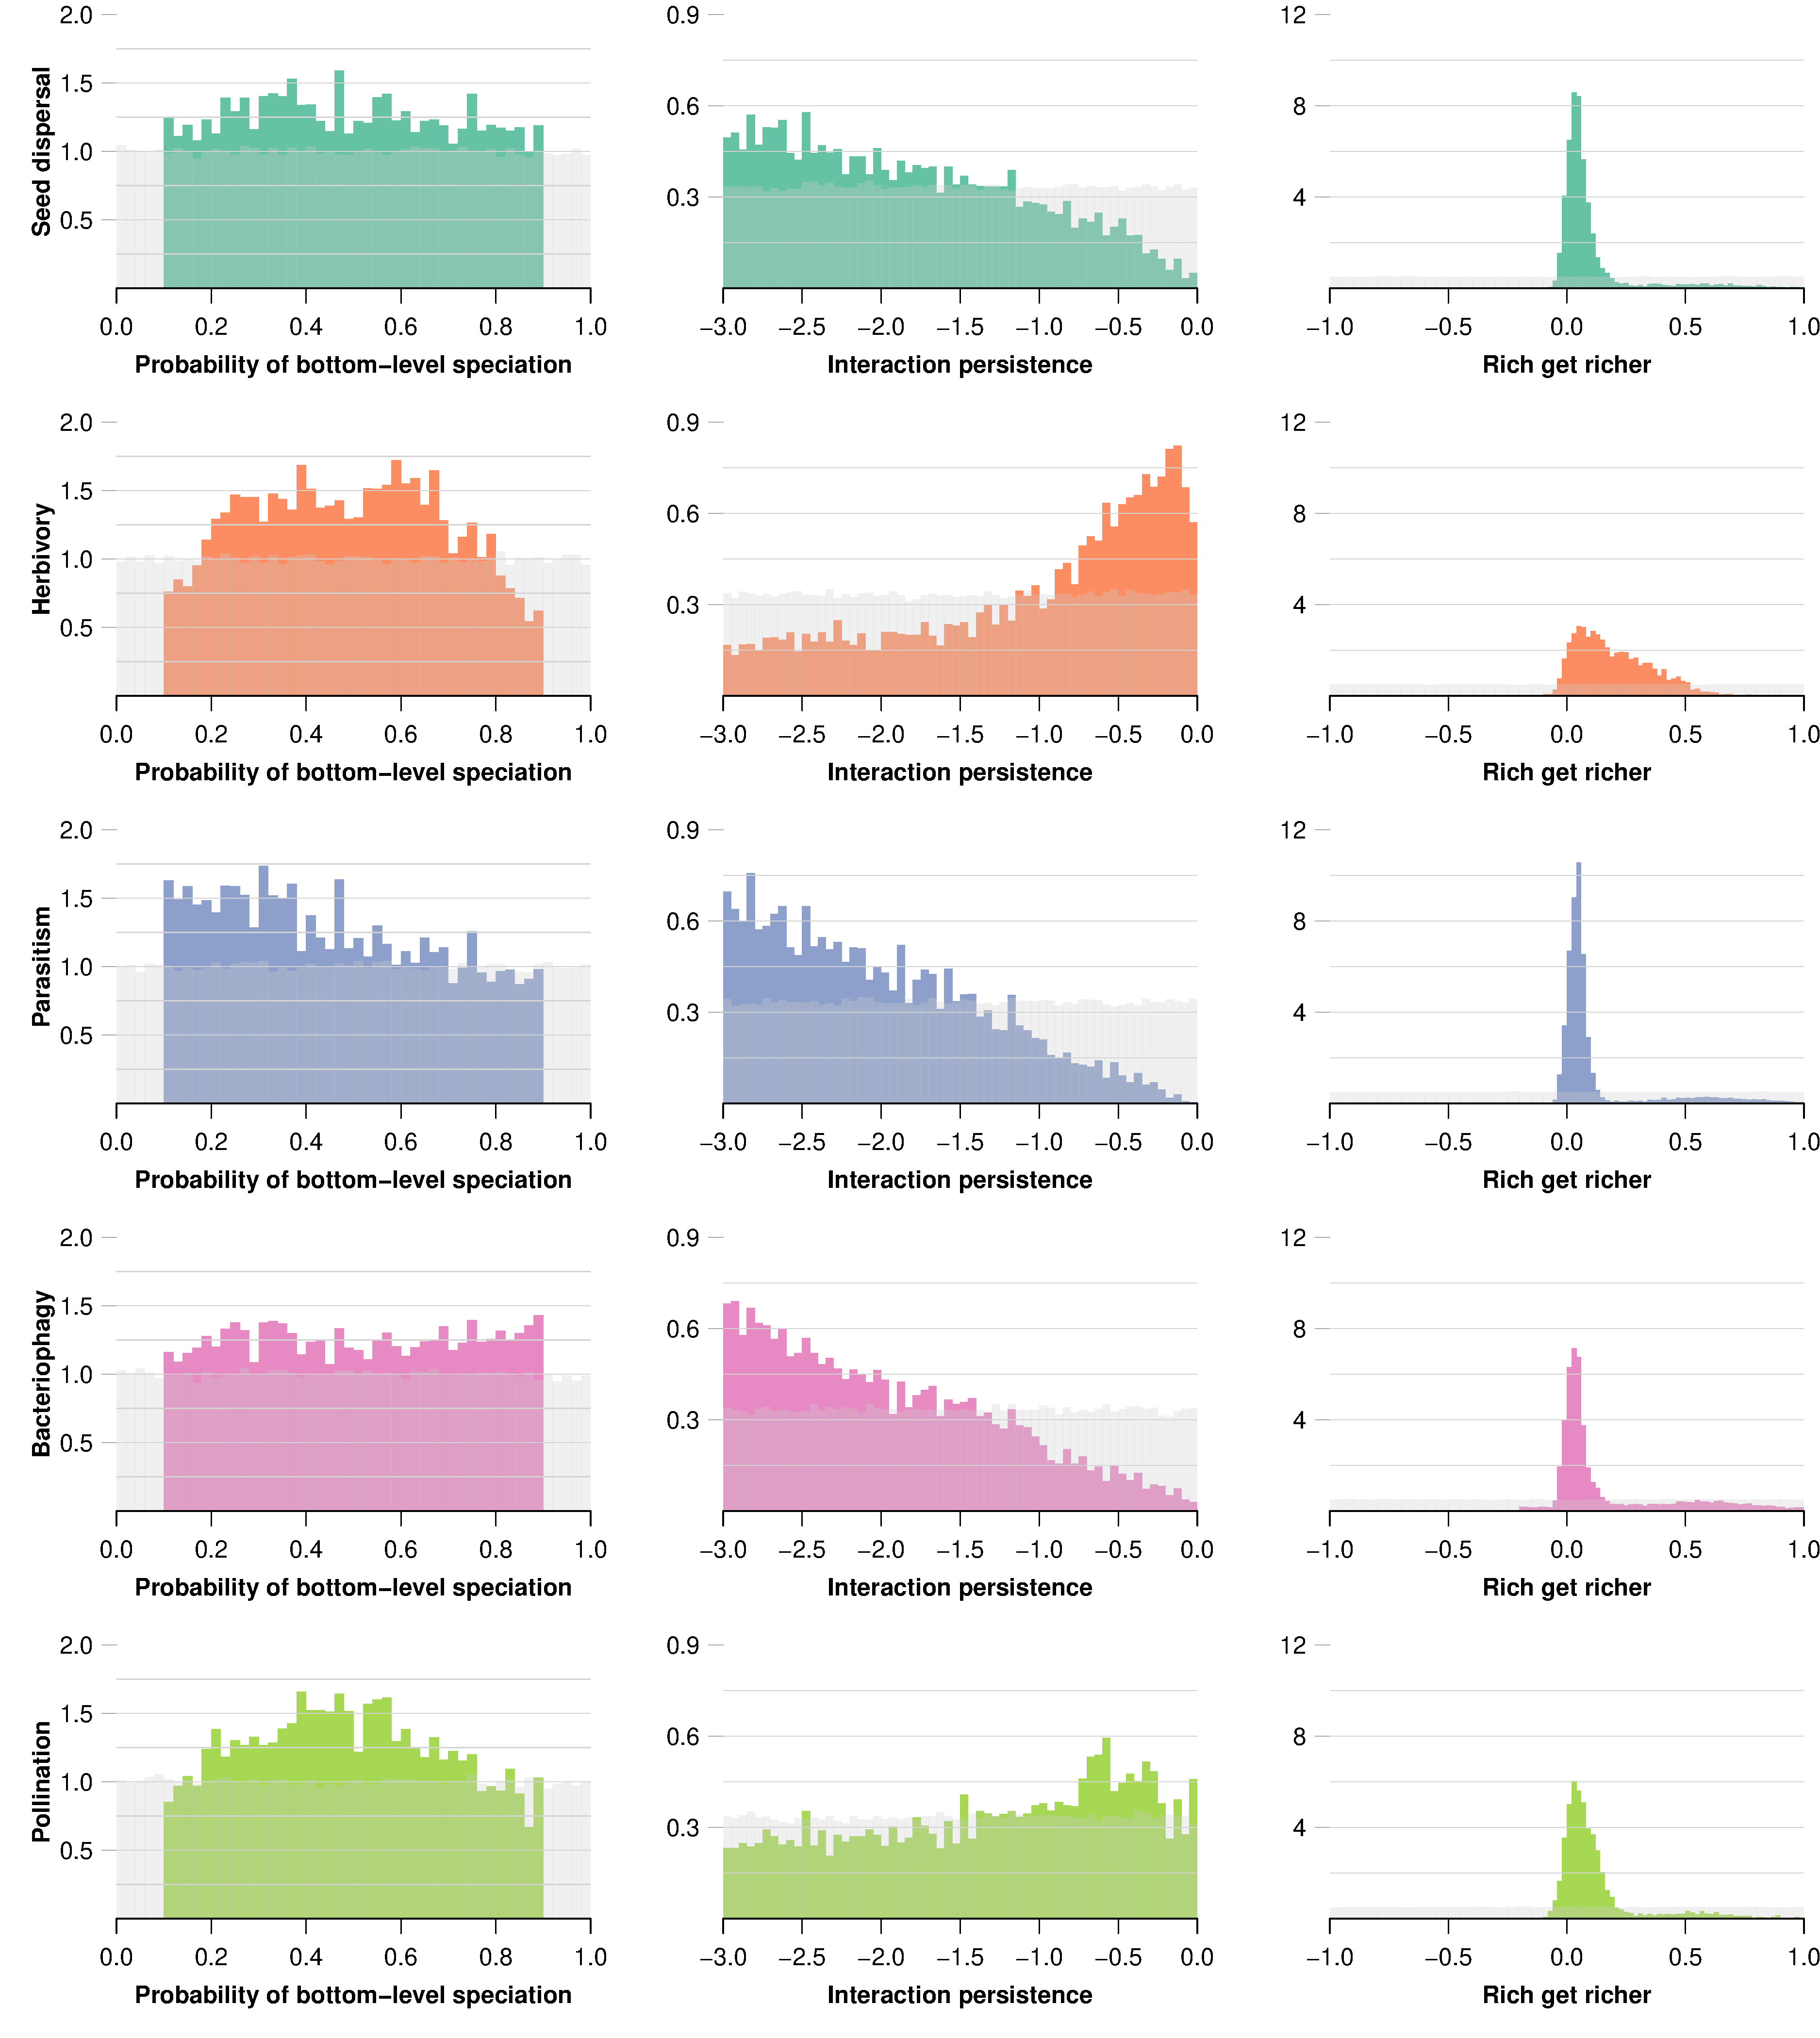
\includegraphics[width=\textwidth]{figures/posteriors.pdf}
    \caption[Posterior distributions of parameters $p$, $\lambda$ and $c$.]{Posterior distributions of parameters $p$, $\text{log}_{10}\lambda$ and $\text{log}_{10}c$. The grey shaded area is a representation of the uniform prior distribution. Although there is no strong selections on the values of $p$, networks do differ strongly both from the prior, and from one another, in terms of $\lambda$ and $c$.}
    \label{posteriors}
\end{figure*}

We first observed that the posterior distribution of the parameters
differs across interaction types (\autoref{posteriors}). The probability
of speciation at either level (\(p\)) is the least strongly selected,
which suggests that mechanisms pertaining to the evolution of
interactions have a stronger impact on extant network structure than
does the distribution of speciation rates. We also encountered two
situations for the distribution of the interaction rate \(\lambda\):
herbivory and pollination networks have higher values of this parameter,
implying that herbivores and pollinators tend to retain the interactions
of their ancestors more than other types of top-level organisms did
(Johnson 2010; Gomez et al. 2013). All other types of networks were best
described by low values of \(\lambda\); their interactions consequently
appear to be more labile throughout the course of macro-evolution.
Finally, all systems show a strong bias towards moderately high values
of \(c\); this indicates that the effective probability of a species
retaining its ancestor's interactions decreases with its ancestor's
degree. That is, the generalism of species over time has an emergent
upper bound, a fact that results in the very spectrum of high-degree and
low-degree species that is ubiquitous empirically (Williams 2011).

The optimal values of \(\lambda\) and \(c\), however, are not
independent since they ultimately affect the same process: the
probability of the incipient species losing its ancestor's interactions.
A more thorough understanding of the dynamics of interactions throughout
evolution can therefore be obtained by examining these parameters' joint
distribution. Doing so reveals two additional ``states'' for networks to
occupy based on the results of our model (\autoref{parameters}); either
\(c\) is close to 0 and \(\lambda\) is large or \(c\) is close to 1 and
\(\lambda\) is low. Notably, different types of networks fall in a
specific place within this continuum. Herbivory and pollination tend to
have both low values of \(c\) and low to high values of
\(\lambda\)---implying that the control on interaction persistence is at
the community level---whereas parasitism networks have low values of
\(\lambda\) and low-to-high values of \(c\)---implying that the control
on interaction persistence is at the species level. The two remaining
network types, seed dispersal and bacteriophagy, do not show a strong
signal as to their position alongside this gradient.

\begin{figure*}[bt]
    \centering
    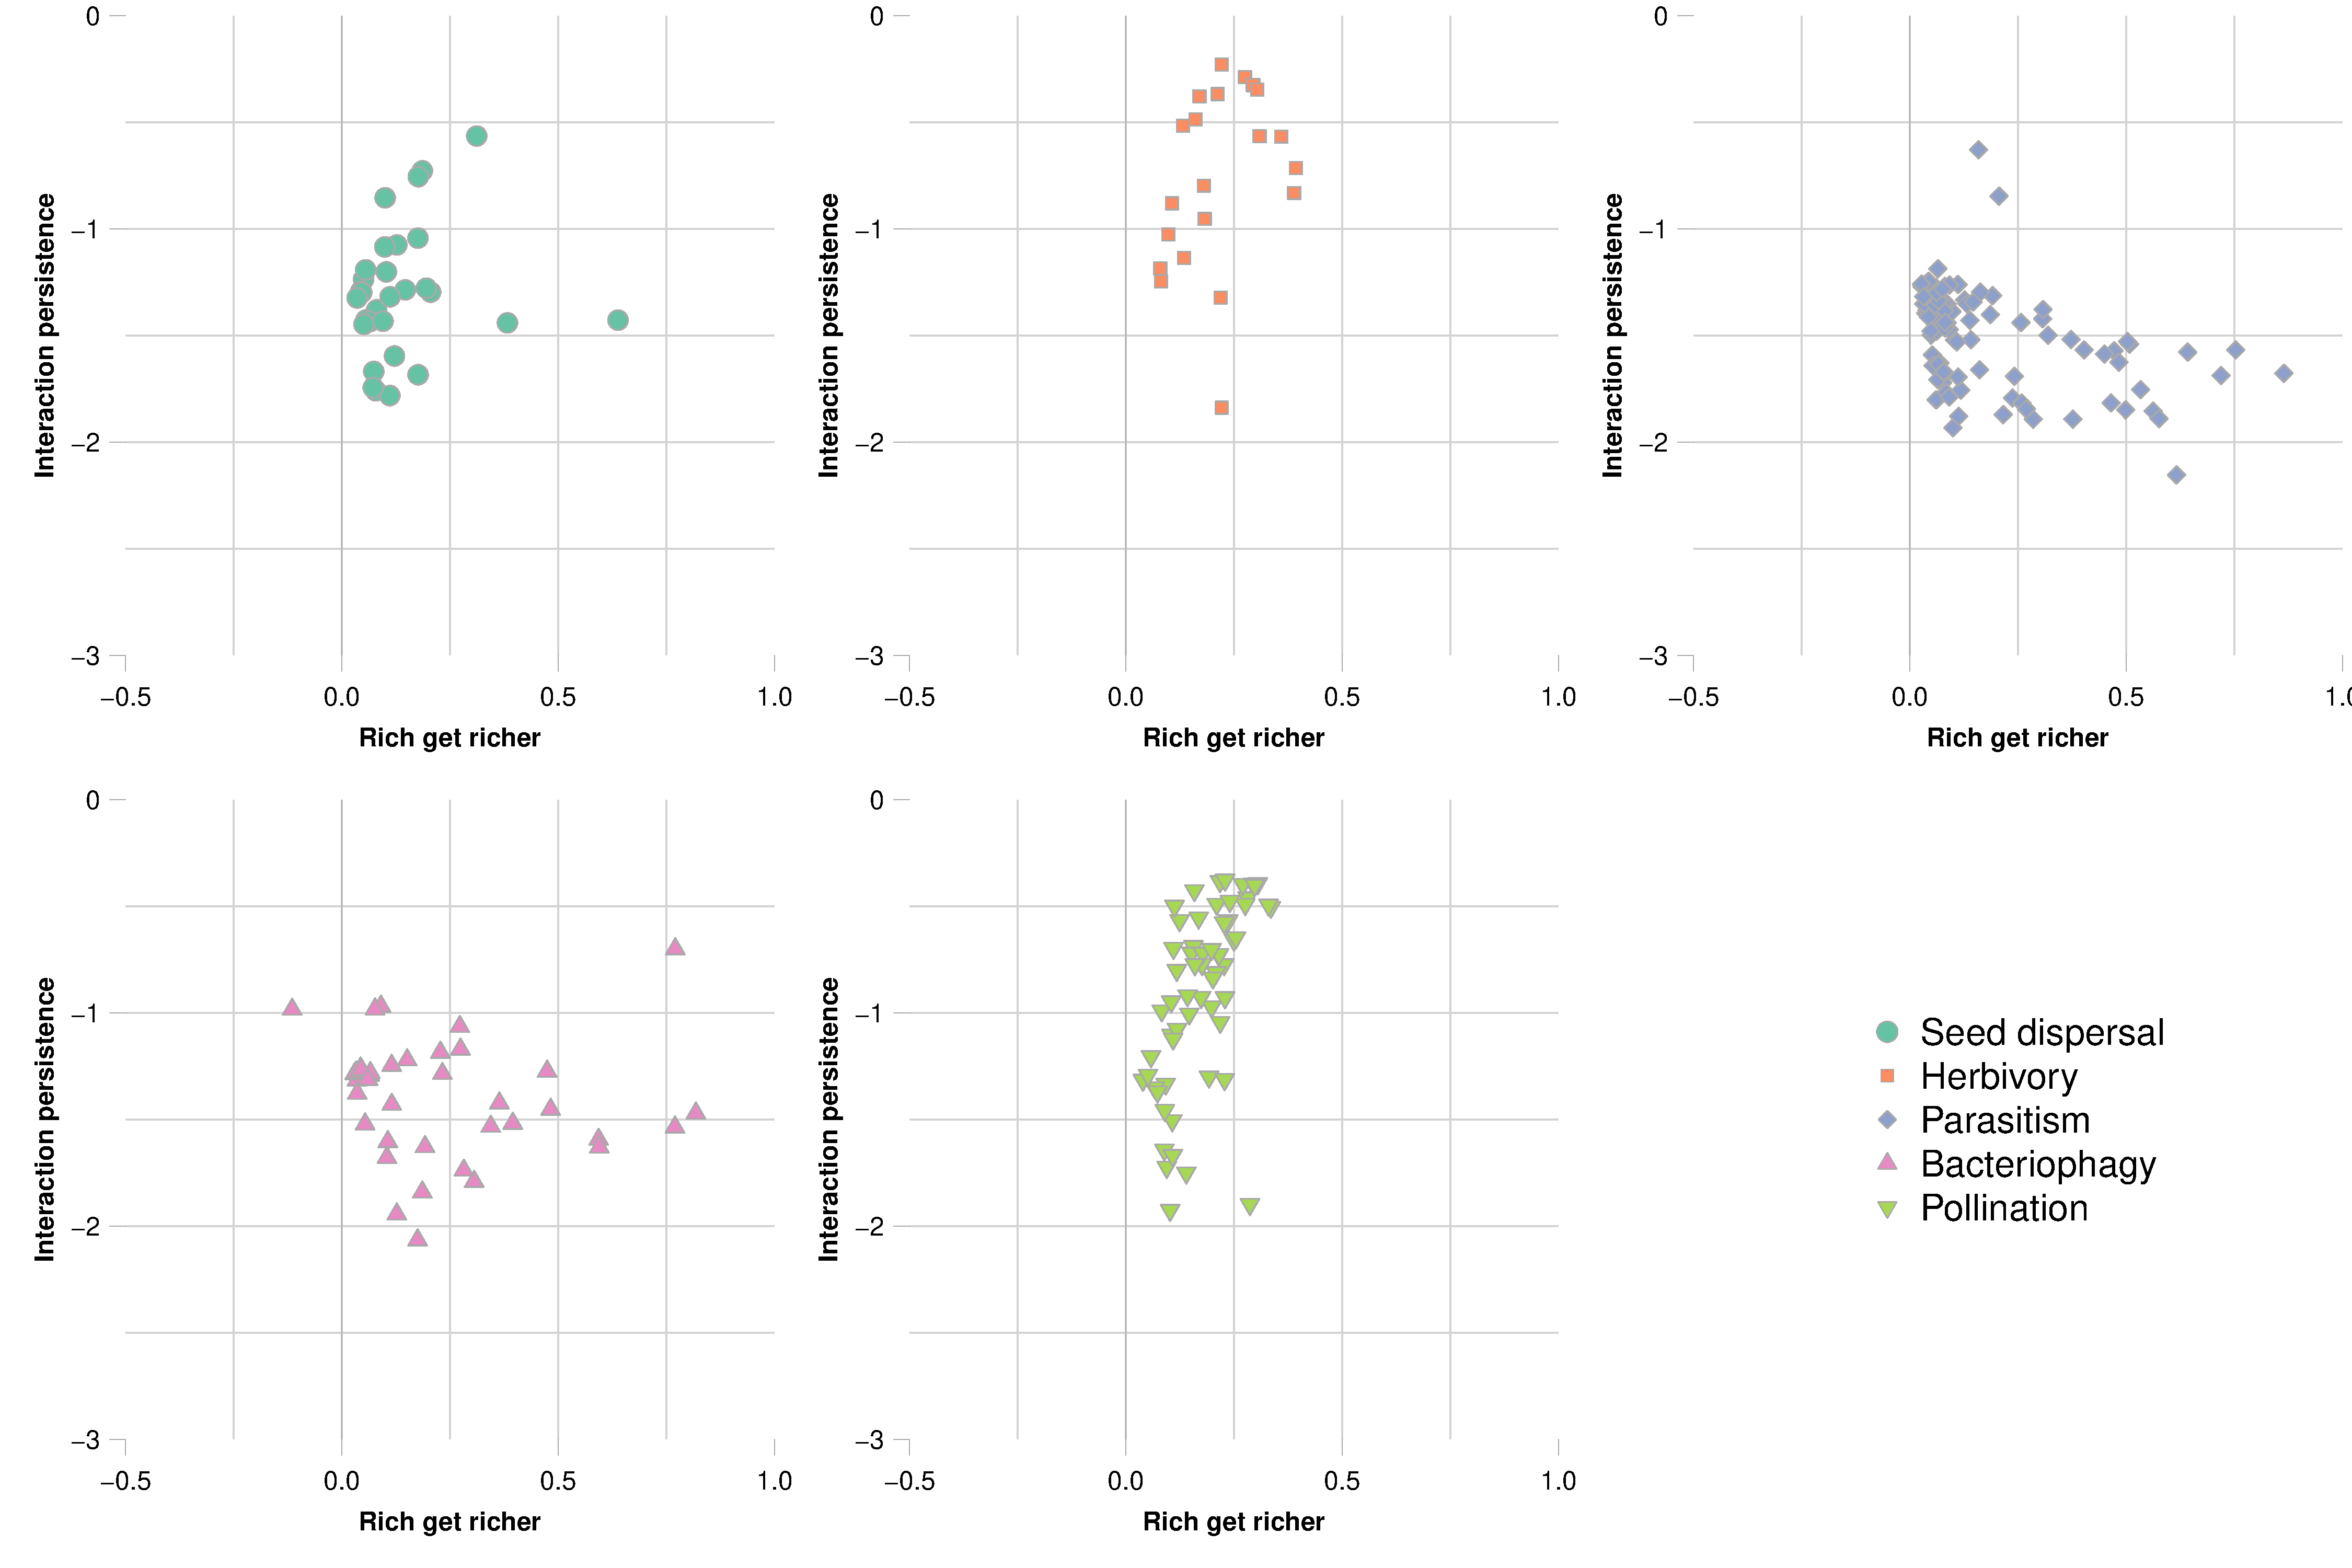
\includegraphics[width=\textwidth]{figures/interaction-params.pdf}
    \caption[Relationships between parameters $\lambda$ and $c$.]{Relationships between parameters $\lambda$ and $c$ in the five different types of networks. It is visually apparent that different types of ecological interactions occupy different positions along the $\lambda$-$c$ continuum.}
    \label{parameters}
\end{figure*}

For each network, we next calculated the average distance to all its
best matching simulation outputs, and used the z-score of this value to
determine which type of networks was best predicted using our model
(\autoref{zscores}). The best predicted networks were herbivory and
pollination; this suggest that these networks have a particularly strong
macro-evolutionary signal (Strauss \& Armbruster 1997).

\begin{figure*}[bt]
    \centering
    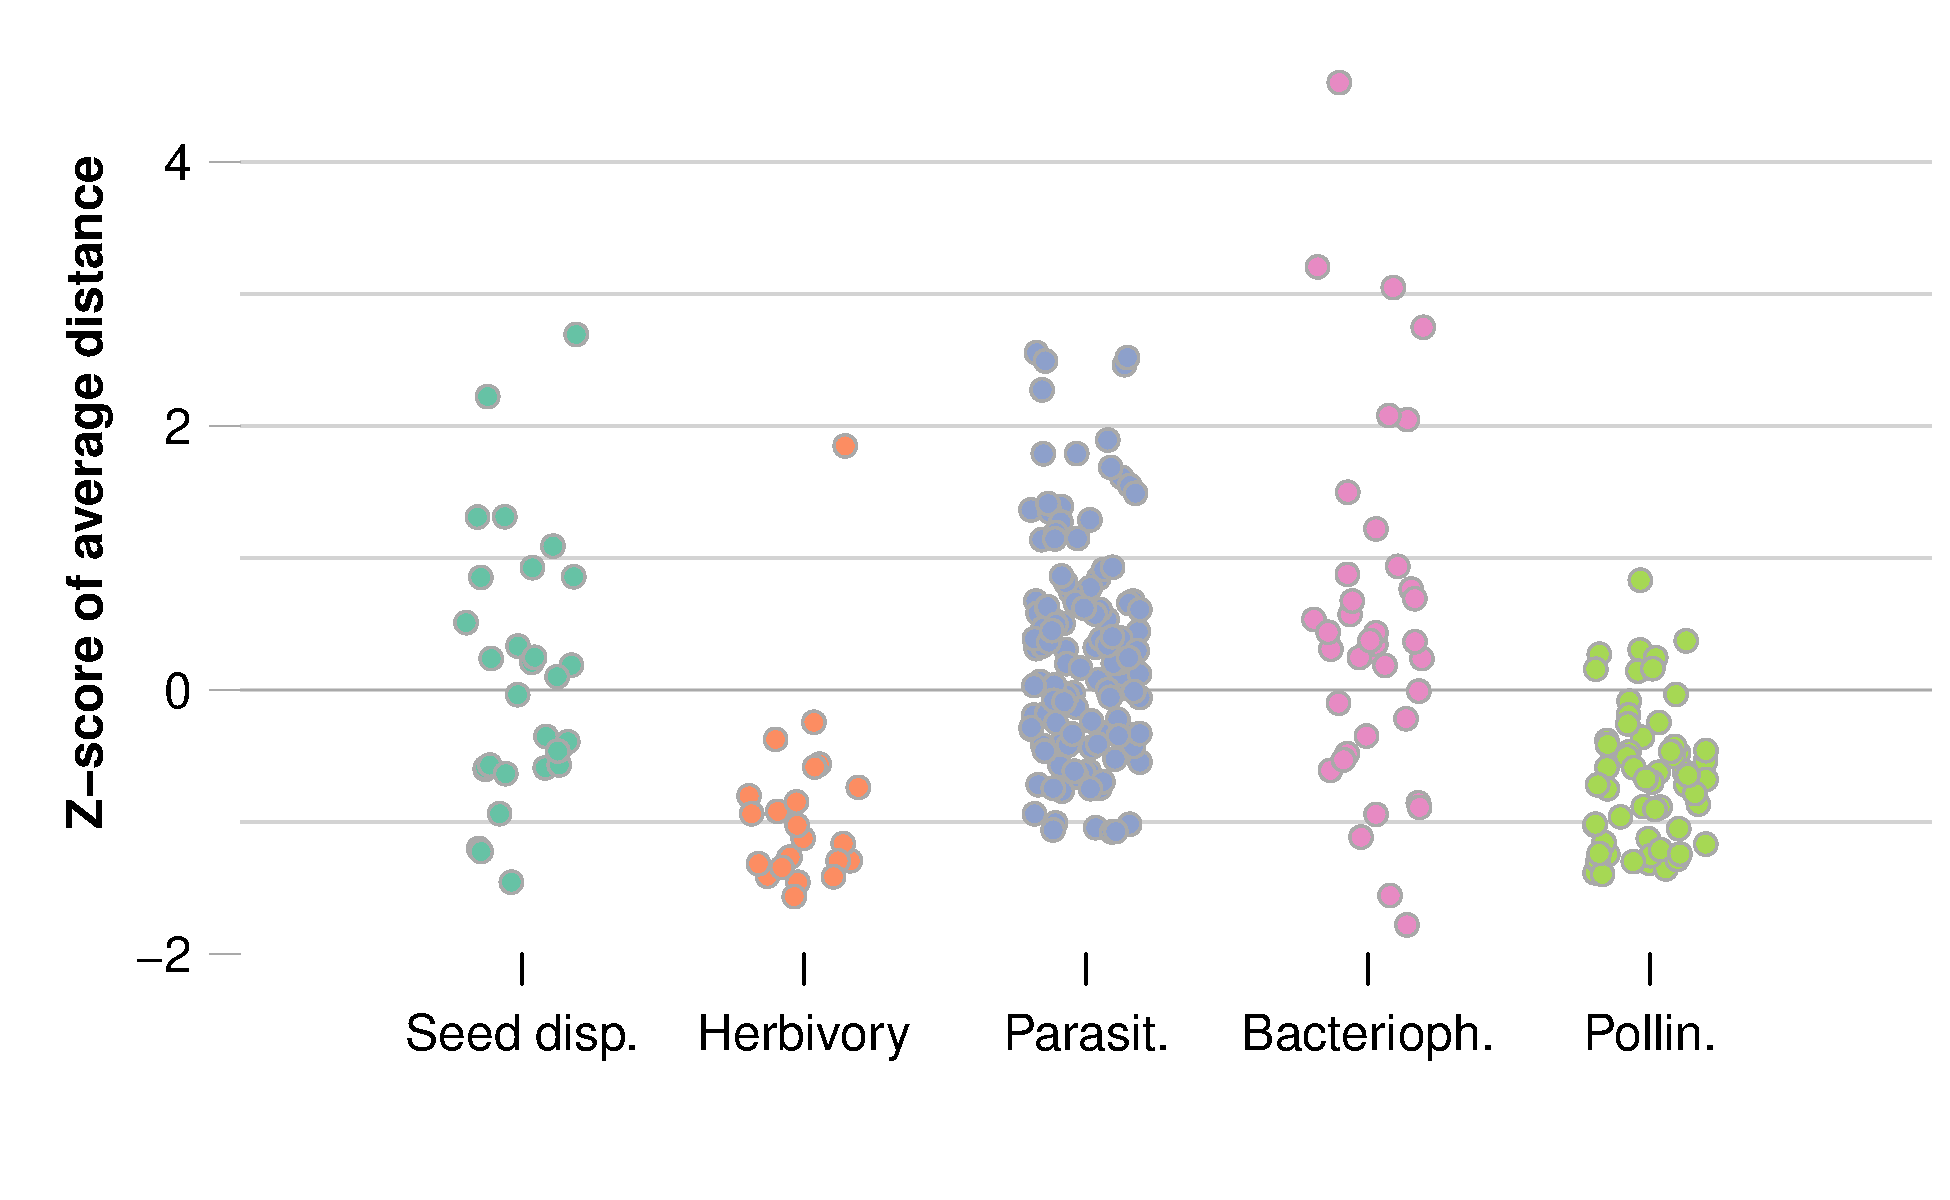
\includegraphics[width=\textwidth]{figures/z-scores.pdf}
    \caption[Predictive power of the model across different types of networks.]{Z-score of average distances for the top 1\% of best-matching simulations. Herbivory and pollination networks are better predicted by this model, while z-scores for seed dispersal, parasitism, and bacteriophagy, are centred around 0. The differences in z-scores may arise for the fact that macro-evolutionary processes have left stronger fingerprint on the extant structure of some types of interactions (\emph{e.g.} herbivory and pollination).}
    \label{zscores}
\end{figure*}

Finally, we applied a classification tree to the parameter values
describing each empirical network (\autoref{tree}). The tree had a
misclassification rate of 35.4\%, meaning that knowing only the value of
parameters \(\lambda\) and \(c\), the correct type of ecological
interaction can be estimated in around 65\% of cases. The structure of
tree also reveals that antagonistic and mutualistic interactions
\emph{do not} form different clusters (as opposed to what has been
hypothesized before; Thébault \& Fontaine 2008), which contradicts the
frequent assumption that different \emph{consequences} of the
interaction should imply different macro-evolutionary rules and
trajectories (Fontaine et al. 2011).

\begin{figure}[bt]
    \centering
    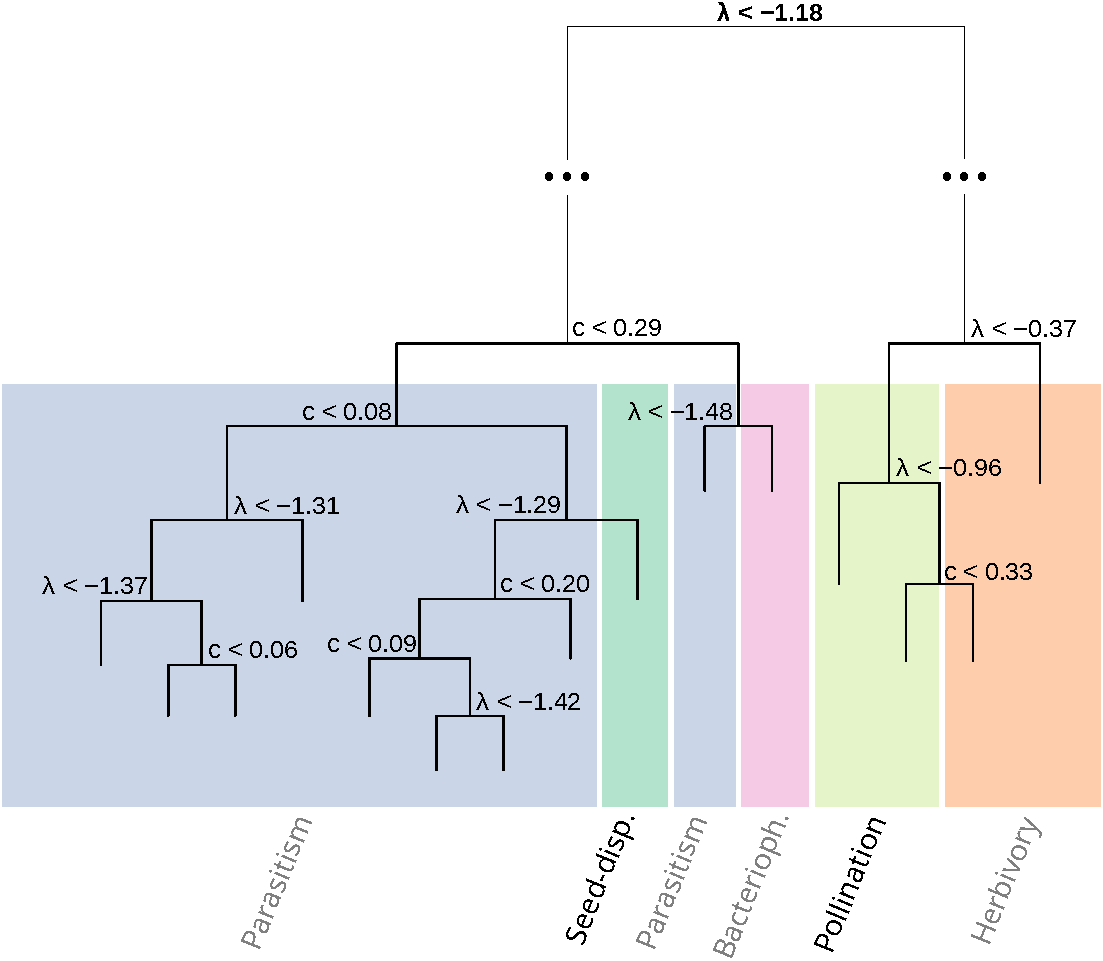
\includegraphics[width=\columnwidth]{figures/tree-cleaned.pdf}
    \caption[Classification tree of the networks as a function of best parameters values.]{Classification tree on parameters $c$ and $\lambda$. Networks are split in two main groups (herbivory and pollination vs others) by $\lambda$. It is worth noting that the groups do not delineate antagonistic (grey labels) from mutualistic (black labels) interactions. Note that the two longest branches have been shortened to improve visual clarity.}
    \label{tree}
\end{figure}

Our results demonstrate that the structure of extant bipartite networks
can be adequately reproduced by a speciation/extinction model that
accounts for biotic interactions. The selection on parameters related to
interaction diversification and persistence was stronger than on the
parameter related to the rate of speciation, suggesting that the
importance of biotic interactions in macro-evolution may have been
understated. Our results also highlight that, while the evolutionary
persistence of interactions is undeniably important in the
macro-evolution of community structure, different type of ecological
interactions respond in largely different ways. This offers a very
stimulating possibility -- namely, that because the mode of coevolution
\emph{within} the interaction between two species differ as a function
of their ecological interactions (Thompson 1994), this can cascade up to
the macro-evolutionary scale in the form of a signal of long-term
interaction persistence.

\section{Methods}\label{methods}

\subsection{Data selection}\label{data-selection}

We used empirical data of plant-pollinator interactions (59 networks),
plant-herbivore interactions (23 networks), phage-bacteria networks (38
interactions), plant-dispersers interactions (30 networks), and
host-parasite interactions (121 networks). Pollination and
seed-dispersal interactions come from the \emph{WebOfLife} dataset
(\texttt{http://mangal.io/data/dataset/7/}). Phage-bacteria (which are
functionally equivalent to host-parasitoid) data are from Flores et al.
(2011). Host-parasite data (Stanko \& Miklisova 2014) are from Canard et
al. (2014). Plant-herbivore data are from Thébault \& Fontaine (2008).
Every network was ``cleaned'' in the following way. First, species with
no interactions (if any) were removed. This yields networks in which all
species have at least one interaction. Second, interactions strengths
(if present) were removed since our model only requires information
about the presence or absence of interactions.

\subsection{Simulations}\label{simulations}

We conducted the following two numerical experiments. First, we
conducted a systematic exploration of the model's behaviour using evenly
spaced parameter values. Each combination of parameters was simulated
1000 times. This allowed us to ensure that the model could return
networks with all possible configurations, and that the output covered a
range of network structures larger than what was observed in nature.
Second, we sampled the parameter space uniformly, by drawing \(10^5\)
parameter sets at random from within the aforementioned bounds. These
outputs were used in the parameter selection experiment described below.

Each timestep in the simulation consists of three sub-steps. First, a
level is picked at random: the top-level is picked with probability
\(p\), and the bottom-level is picked with probability \(1-p\). This is
independent of the number of species at each level. Second, one species
from the selected level is picked at random (all species within a level
have equal chance of being picked), and duplicated (\emph{i.e.} a novel
species with the same interactions is added to the network). Each
interaction of the incipient species is then \emph{removed} with
probability

\begin{equation}
\epsilon(\lambda, k, c) = \frac{1}{1+\left(\frac{1}{\lambda}-1\right)\times c^{k-1}} \,.
\end{equation}

In this formulation, \(k\) is the number of interactions of the
incipient species, \(\lambda\) is the \emph{basal} rate of interaction
loss, and \(c\) is a parameter regulating whether species with more
interactions tend to gain or lose interactions over time. Negative
values of \(c\) imply that \emph{rich get richer}, \emph{i.e.} species
with more interactions tend to conserve them more over speciation. The
special case of \(c = 0\) corresponds to no relationship between the
degree of a species and its probability of losing or retaining an
interaction over speciation.

We ran the model for \(10^4\) timesteps, for \(10^5\) random
combinations of \(<p, \lambda, c>\). Whenever either level has more than
\(10^2\) species, some are deleted at random within this level. This
ensure that the network is at most composed of 200 species. Preliminary
analyses revealed that this threshold had no impact on the results
presented as long as it was reasonably large (\(\geq 50\)).

\subsection{Network measures}\label{network-measures}

We measured four key families of bipartite network structure indices. To
facilitate their use in distance calculations, we transformed all
measures so that they fell in the range \([0,1]\). First, connectance,
which is the \(\frac{L}{T\times B}\), with \(L\) the number of
interactions, and \(T\) and \(B\) the number of species in the top and
bottom groups. Second, nestedness (Almeida-Neto et al. 2008), using the
\(\eta\) measure of Bastolla et al. (2009), which returns a global
nestedness score based on the fact that interactions of relatively
specialized species should be a subset of the interactions of more
generalized ones. Third, modularity, using LP-BRIM (Barber 2007; Liu \&
Murata 2009), which gives values close to 1 when there are modules in
the network, and values closer to 0 otherwise. Finally, we measured the
proportion of all four-species bipartite motifs (Baker et al. 2014).
Bipartite motifs are all the possible conformations of four species
spread across two levels, such as for example three consumers sharing
one resource, or two consumers both exploiting resources, \emph{etc.}.

So that the motif measure would also fall in the range \([0,1]\), we
corrected the raw number of motifs to account for the number of species
in each layer of the bipartite network. For example, the maximum number
of motifs with 2 species at the top and 2 species at the bottom is the
product of the number of combinations of 2 species in the top layer, and
of 2 species in the bottom layer (evaluated by their binomial
coefficients \({T \choose 2}\) and \({B \choose 2}\), respectively).
This gives a total number of sets of species that \emph{could} be
involved in a \(2 \times 2\) motif. Note that this implies that all
values represent the proportion of sets of species that \emph{do} form a
given motif out of the sets of species that \emph{could}.

\subsection{Parameter selection}\label{parameter-selection}

We used ABC (Approximate Bayesian Computation) to select the parameter
values that yielded realistic networks by assessing how closely each
replicate of the second numerical experiment resembles empirical
communities. For each empirical network, its observed set of summary
statistics was compared to each output of the stochastic model. The
inverse of the Euclidean distance between the two arrays was recorded as
the score of the parameter set. Because each empirical network is in
practice a different optimization problem submitted to the ABC routine,
and because ABC requires to set the rejection threshold on a per-problem
basis, setting a global value was not meaningful. To circumvent this
problem, we instead selected the posterior distribution as the 500
parameters sets that gave the best scores (\emph{i.e.} above the 95th
percentile). The distribution of distances (\emph{i.e.} how well each
point within the posterior distributions actually describes the
empirical network) is kept to evaluate the global fit on a per-network
basis.

\subsection{Decision tree}\label{decision-tree}

We used a classification tree to separate the networks along the
continuum of values of \(c\) and \(\lambda\). The response was the type
of network, and the classifiers where the \(\text{log}_{10}\) of \(c\)
and \(\lambda\) and the log transformation helped do something real and
spectacular. We used the implementation from the \texttt{tree} package
(v. 1.0.36) for \texttt{R} (v. 3.2.2). Splits where decided according to
Gini ratio. The weight of each datapoint was proportional to the inverse
of the Euclidean distance between the output of the simulation and the
actual network, so that networks that were poorly described by the model
have a lessened impact on the classification.

\section*{References}\label{references}
\addcontentsline{toc}{section}{References}

\hypertarget{refs}{}
\hypertarget{ref-alme08cmn}{}
\textbf{Almeida-Neto et al.} (2008). A consistent metric for nestedness
analysis in ecological systems: reconciling concept and measurement.
\emph{Oikos.} 117:1227--39.

\hypertarget{ref-alro98crd}{}
\textbf{Alroy}. (1998). Cope's Rule and the Dynamics of Body Mass
Evolution in North American Fossil Mammals. \emph{Science.} 280:731--4.

\hypertarget{ref-bake14srf}{}
\textbf{Baker et al.} (2014). Species' roles in food webs show fidelity
across a highly variable oak forest. \emph{Ecography.} 38:130--9.

\hypertarget{ref-barb07mcd}{}
\textbf{Barber}. (2007). Modularity and community detection in bipartite
networks. \emph{Physical Review E.} 76.

\hypertarget{ref-bast09amn}{}
\textbf{Bastolla et al.} (2009). The architecture of mutualistic
networks minimizes competition and increases biodiversity.
\emph{Nature.} 458:1018--20.

\hypertarget{ref-beau10abc}{}
\textbf{Beaumont}. (2010). Approximate Bayesian Computation in Evolution
and Ecology. \emph{Annu Rev Ecol Evol Syst.} 41:379--406.

\hypertarget{ref-bock72sim}{}
\textbf{Bock}. (1972). Species Interactions and Macroevolution.
\emph{Evolutionary Biology.} Springer Science + Business Media; pp.
1--24.

\hypertarget{ref-cana14een}{}
\textbf{Canard et al.} (2014). Empirical Evaluation of Neutral
Interactions in Host-Parasite Networks. \emph{The American Naturalist.}
183:468--79.

\hypertarget{ref-csil10abc}{}
\textbf{Csilléry et al.} (2010). Approximate Bayesian Computation (ABC)
in practice. \emph{Trends in Ecology \& Evolution.} 25:410--8.

\hypertarget{ref-eklo11reh}{}
\textbf{Eklof et al.} (2011). Relevance of evolutionary history for food
web structure. \emph{Proceedings of the Royal Society B: Biological
Sciences.} 279:1588--96.

\hypertarget{ref-eklo13den}{}
\textbf{Eklöf et al.} (2013a). The dimensionality of ecological
networks. \emph{Ecology Letters.} 16:577--83.

\hypertarget{ref-eklo13sef}{}
\textbf{Eklöf et al.} (2013b). Secondary extinctions in food webs: a
Bayesian network approach. \emph{Methods Ecol Evol.} 4:760--70.

\hypertarget{ref-flor11ssh}{}
\textbf{Flores et al.} (2011). Statistical structure of host-phage
interactions. \emph{Proceedings of the National Academy of Sciences.}
108:E288--97.

\hypertarget{ref-font11eei}{}
\textbf{Fontaine et al.} (2011). The ecological and evolutionary
implications of merging different types of networks. \emph{Ecology
Letters.} 14:1170--81.

\hypertarget{ref-fort10nvm}{}
\textbf{Fortuna et al.} (2010). Nestedness versus modularity in
ecological networks: two sides of the same coin? \emph{Journal of Animal
Ecology.}

\hypertarget{ref-futu09ehs}{}
\textbf{Futuyma \& Agrawal}. (2009). Evolutionary history and species
interactions. \emph{Proceedings of the National Academy of Sciences.}
106:18043--4.

\hypertarget{ref-gome13epn}{}
\textbf{Gomez et al.} (2013). Evolution of pollination niches and floral
divergence in the generalist plant Erysimum mediohispanicum.
\emph{Annals of Botany.} 113:237--49.

\hypertarget{ref-grav11tti}{}
\textbf{Gravel et al.} (2011). Trophic theory of island biogeography.
\emph{Ecology Letters.} 14:1010--6.

\hypertarget{ref-jabl08bim}{}
\textbf{Jablonski}. (2008). BIOTIC INTERACTIONS AND MACROEVOLUTION:
EXTENSIONS AND MISMATCHES ACROSS SCALES AND LEVELS. \emph{Evolution.}
62:715--39.

\hypertarget{ref-john10pnr}{}
\textbf{Johnson}. (2010). The pollination niche and its role in the
diversification and maintenance of the southern African flora.
\emph{Philosophical Transactions of the Royal Society B: Biological
Sciences.} 365:499--516.

\hypertarget{ref-liu09cdl}{}
\textbf{Liu \& Murata}. (2009). Community Detection in Large-Scale
Bipartite Networks. \emph{2009 IEEE/WIC/ACM International Joint
Conference on Web Intelligence and Intelligent Agent Technology.}
Institute of Electrical \& Electronics Engineers (IEEE);

\hypertarget{ref-nee06bmm}{}
\textbf{Nee}. (2006). Birth-Death Models in Macroevolution. \emph{Annu
Rev Ecol Evol Syst.} 37:1--17.

\hypertarget{ref-oles07mpn}{}
\textbf{Olesen et al.} (2007). The modularity of pollination networks.
\emph{Proceedings of the National Academy of Sciences.} 104:19891--6.

\hypertarget{ref-pera16meh}{}
\textbf{Peralta}. (2016). Merging evolutionary history into species
interaction networks. \emph{Functional Ecology.}

\hypertarget{ref-roop06ecc}{}
\textbf{Roopnarine}. (2006). Extinction cascades and catastrophe in
ancient food webs. \emph{Paleobiology.} 32:1--19.

\hypertarget{ref-stan14dee}{}
\textbf{Stanko \& Miklisova}. 2014. Data from: Empirical evaluation of
neutral interactions in host-parasite networks {[}Internet{]}. \emph{The
American Naturalist.} Dryad Digital Repository;

\hypertarget{ref-stou07eer}{}
\textbf{Stouffer et al.} (2007). Evidence for the existence of a robust
pattern of prey selection in food webs. \emph{Proceedings of the Royal
Society B: Biological Sciences.} 274:1931--40.

\hypertarget{ref-stou12ecs}{}
\textbf{Stouffer et al.} (2012). Evolutionary Conservation of Species'
Roles in Food Webs. \emph{Science.} 335:1489--92.

\hypertarget{ref-stra97lhp}{}
\textbf{Strauss \& Armbruster}. (1997). Linking Herbivory and
Pollination--New Perspectives on Plant and Animal Ecology and Evolution.
\emph{Ecology.} 78:1617.

\hypertarget{ref-stro13arc}{}
\textbf{Strotz \& Allen}. (2013). Assessing the role of cladogenesis in
macroevolution by integrating fossil and molecular evidence.
\emph{Proceedings of the National Academy of Sciences.} 110:2904--9.

\hypertarget{ref-theb08asd}{}
\textbf{Thébault \& Fontaine}. (2008). Does asymmetric specialization
differ between mutualistic and trophic networks? \emph{Oikos.}
0:080227085440234--0.

\hypertarget{ref-thom94cp}{}
\textbf{Thompson}. (1994). The Coevolutionary Process {[}Internet{]}.
University of Chicago Press;

\hypertarget{ref-thom12fwr}{}
\textbf{Thompson et al.} (2012). Food webs: reconciling the structure
and function of biodiversity. \emph{Trends in Ecology \& Evolution.}
27:689--97.

\hypertarget{ref-thui13rmi}{}
\textbf{Thuiller et al.} (2013). A road map for integrating
eco-evolutionary processes into biodiversity models. \emph{Ecology
Letters.} 16:94--105.

\hypertarget{ref-will11bmc}{}
\textbf{Williams}. (2011). Biology, Methodology or Chance? The Degree
Distributions of Bipartite Ecological Networks. \emph{PLoS ONE.}
6:e17645.

\end{document}
